\documentclass[AMA,STIX1COL]{WileyNJD-v2}

\articletype{Article Type}%

\usepackage{setspace}


\newcommand{\E}{\mbox{E}}
\newcommand{\RF}{\mbox{RF}}
\newcommand{\Ebar}{\overline{\mbox{E}}}
\newcommand{\RFbar}{\overline{\mbox{RF}}}
\newcommand{\boldtheta}{\boldsymbol{\theta}}
\newcommand{\boldgamma}{\boldsymbol{\gamma}}

\raggedbottom


\begin{document}

\title{Spike-and-Slab Prior Distributions in Bayesian Logistic Meta-analysis}

\author[1]{Thomas A. Gibson*}

\author[1]{Robert E. Weiss}


\authormark{GIBSON, WEISS}


\address[1]{\orgdiv{Department of Biostatistics}, \orgname{University of California, Los Angeles}, \orgaddress{\state{California}, \country{USA}}}


\corres{*Thomas A. Gibson \email{tommy.a.gibson@gmail.com}}

\abstract[Summary]{}

\keywords{keywords}

%\jnlcitation{\cname{%
%\author{Williams K.}, 
%\author{B. Hoskins}, 
%\author{R. Lee}, 
%\author{G. Masato}, and 
%\author{T. Woollings}} (\cyear{2016}), 
%\ctitle{A regime analysis of Atlantic winter jet variability applied to evaluate HadGEM3-GC2}, \cjournal{Q.J.R. Meteorol. Soc.}, \cvol{2017;00:1--6}.}

\maketitle

\footnotetext{\textbf{Abbreviations:} CTS, contingency table statistic; RF, risk factor; IRF, interferon regulatory factor}

\doublespacing

\section{Introduction} \label{sec:intro}


Data from medical studies can often be tabulated appropriately in a 2$\times$2 contingency table. The tables have columns stratified by a dichotomous outcome and rows stratified by a dichotomous covariate. Summary statistics from a 2$\times$2 contingency table include positive/negative predictive value (PPV/NPV), sensitivity and specificity, and positive and negative likelihood ratios (LR+/LR-), among others. We will refer to any statistic that can be calculated as functions of some or all of the four values in a 2$\times$2 contingency table as a \textit{contingency table statistic} (CTS). For an individual study's table, this would mean using the counts in each cell, and for a population it would mean using the underlying multinomial cell probabilities. CTS's describe the relationship between the outcome and the covariate, and calculating most CTS's requires conditioning on either rows or columns. Meta-analysis methods for contingency table data reflect this conditioning, and differ based on the statistics of interest. 

There are two types of meta-analysis models for 2$\times$2 data. The first type models CTS's that condition on the presence (RF) or absence $(\RFbar)$ of a risk factor, while the second type models CTS's that condition on the presence (E) or absence $(\Ebar)$ of an adverse event. CTS's conditioning on RF, which we refer to as \textit{row-CTS's}, include the odds ratio (OR), relative risk (RR), risk difference (RD), and positive/negative predictive values (PPV/NPV). A standard random effects model for row-CTS's is given in \citet{smith1995}, with the log-odds ratio $\log(\mbox{OR})$ as the main inference target. \citet{warn2002} provides a model to explicitly model both RRs and RDs. These methods condition on group $j = 0, 1$ where $j=1$ when the RF is present and $j=0$ when it is absent, and use binomial likelihoods, where the number of events $y_{ij}$ in study $i, i = 1, \dots, S$, group $j$ depends on the number of people $n_{ij}$ in study $i$, group $j$, and the probability of an event in that group, $\pi_{ij}$. CTS's conditioning on E, which we call \textit{column-CTS's}, include sensitivity, specificity, ORs, and positive/negative likelihood ratios (LR+/LR-). \citet{ma2016} reviews models that condition on event status, including the summary receiver operating characteristic (SROC) curve \citep{rutter2001, moses1993} and bivariate random effects models \citep{reitsma2005, chu2006, arends2008}, which use binomial likelihoods to model $\mbox{P}(\E \vert \RF)$ and $\mbox{P}(\E \vert \RFbar)$. 

An area of medical literature particularly suited to generating 2$\times$2 data is emergency department (ED) visits for syncope (fainting), where around 5-10\% of older syncope patients experience an adverse event in the 30 days after their initial ED visit \citep{gibson2018}. Many studies provide 2$\times$2 tables of counts for dichotomous covariates that are regularly collected during an ED visit for syncope patients, including comorbidities, symptoms, and test characteristics. The syncope data is \textit{observational data} (OD), where neither row totals or column totals are fixed by study investigators. For OD we are interested in both row- and column-CTS's. We would also like to ``weed out" those covariates that do not have diagnostic value in predicting adverse events. 

To estimate row- and column-CTS's together we propose a novel Bayesian meta-analysis model with 3 random effects (3 RE) as an extension of the model in \citet{smith1995}, with random effects on the log-odds of an event, the $\log(\mbox{OR})$, and the log-odds of having the risk factor. By modeling these three factors together we can make inference on both row- and column-CTS's. The model proposed by \citet{chu2009} models the probability of a positive diagnostic test simultaneously with sensitivity and specificity, which enables the user to obtain estimates of PPV and NPV. We use a fully Bayesian approach which has advantages in interpretation and flexibility. Additionally, the model in \citet{chu2009} estimates medians for both study-specific and global parameters. Within our Bayesian approach we can easily calculate means of study-specific parameters and we define a novel estimand for global parameters, the expected value of a given statistic for a new study, which accounts for all appropriate variability, and we outline a procedure to sample from the posterior distribution of the estimand. 

Determining which covariates have no diagnostic value corresponds to a natural scientific question in random effects meta-analysis of whether or not the mean effect size $\log(\mbox{OR})$ for a given covariate is different from zero \citep{higgins2009}. Classical meta-analyses take a hypothesis testing approach, using Wald statistics \citep{higgins2009, follmann1999} or a maximum likelihood model proposed by \citet{hardy1996}, which accounts for uncertainty in the estimation of heterogeneity parameters. 

We introduce a mixture spike-and-slab prior distribution \citep{GM1993, GM1997, KM1998, ishwaran2005} on the mean parameter for random effects on the $\log(\mbox{OR})$ in the 3 RE model, which allows us to calculate the posterior probability that the null hypothesis is true. The mixture prior places point mass on the probability that the mean $\log(\mbox{OR}) = 0$ (the spike), and if not 0, models uncertainty in the mean $\log(\mbox{OR})$ with a continuous prior distribution (the slab). To our knowledge, spike-and-slab priors have not been used in the Bayesian meta-analysis literature. 

We present the 3 RE meta-analysis model and detail where a spike-and-slab prior can be used in Section \ref{sec:methods}. Section \ref{sec:simulation} presents a simulation. Section \ref{sec:syncope} illustrates in application to syncope data. The paper closes with a discussion. 

\section{Three RE meta-analysis model} \label{sec:3REmodel}

In the usual meta-analysis, each paper $i = 1, \dots, S$ in the meta-analysis provides a 2$\times$2 table with rows defined by the presence (RF), $j = 1$, or absence ($\RFbar$), $j = 0$, of a risk factor and columns defined by adverse event (E) or no adverse event ($\Ebar$). Let $N_i = n_{i0} + n_{i1}$ be the total sample size in study $i$, where $n_{ij}$ is the number of people in study $i$, group $j=0,1$, $y_{ij}$ be the number of people with an adverse event in study $i$, group $j$, and $\pi_{ij}$ be the probability of an adverse event for a patient in study $i$, group $j$ as illustrated in Table \ref{table:RCT_contingency}. Assuming binomial sampling, the standard Bayesian random effects meta-analysis model is 
\begin{align}
y_{ij} \vert \pi_{ij} & \sim \mbox{Bin}(n_{ij}, \pi_{ij})  \label{eq:likelihood}\\
\mbox{logit}(\pi_{ij}) & =  \left\{
                  \begin{array}{ll}
                    \beta_{i} - \frac{\delta_i}{2} & \quad j=0 \\ 
                    \beta_{i} + \frac{\delta_i}{2} & \quad j=1,
                  \end{array}
                \right. \label{eq:logit}
\end{align}

\noindent where $\mbox{logit}(a) = \log(a/(1-a))$, $\beta_i$ is a random intercept term for the log-odds of the event for study $i$ and $\delta_i$ is a random effect for the $\log(\mbox{OR})$ of the event in study $i$. Giving each study its own $\beta_i$ allows the log-odds of an event to be different for each study $i$, as we might expect due to population and methodology differences between studies, and giving each study its own $\delta_i$ models a random study by RF interaction effect. We model $\delta_i$ and $\beta_i$ as normal
\begin{align}
\delta_i \vert \delta_0, \sigma^2_{\delta} & \sim \mbox{N}(\delta_0, \sigma^2_{\delta}) \label{eq:deltai} \\
\beta_i \vert \beta_0, \sigma^2_{\beta} & \sim \mbox{N}(\beta_0, \sigma^2_{\beta}), \label{eq:betai}
\end{align}
\noindent and unknown hyperparameters for the mean $\log(\mbox{OR})$ $\delta_0$, mean $\log(\mbox{odds})$ of the event $\beta_0$,  variance of $\log(\mbox{OR})$'s $\sigma^2_{\delta}$, and variance in $\log(\mbox{odds})$ of the event $\sigma^2_{\beta}$ have appropriate prior distributions which we discuss in Section \ref{sec:priors}. 

We now expand \eqref{eq:likelihood} - \eqref{eq:betai} and add a random effect $\psi_i = \mbox{P}(\RF_{ij}$, the probability of having the risk factor for subject $j$ in study $i$. Defining $\nu_i = \mbox{logit}(\psi_i)$, we assume binomial sampling for $n_{i1}$ from $N_i$ and model $\nu_i$ as normal
\begin{align}
n_{ij} \vert \psi_i &\sim \mbox{Bin}(N_i, \psi_i) \label{eq:nij} \\
\nu_i \vert \nu_0, \sigma^2_\nu & \sim \mbox{N}(\nu_0, \sigma^2_\nu), \label{eq:nui}
\end{align}
\noindent where the unknown hyperpriors $\nu_0$ and $\sigma^2_\nu$ have priors $f(\nu_0)$ and $f(\sigma^2_{\nu})$. 

\subsection{Estimating contingency table statistics} \label{sec:CTSs}

We can calculate two versions of each CTS: study-specific and \textit{global}. Let $\boldsymbol{Y}$ be the data from all $S$ studies and let $\boldtheta_i = (\beta_i, \delta_i, \nu_i)$ be the vector of study-specific parameters. The unknown study-specific CTS$_i$'s are functions of
\begin{align}
\pi_{i1} &= \mbox{expit}(\beta_i + \delta_i / 2) \nonumber \\
\pi_{i0} &= \mbox{expit}(\beta_i - \delta_i / 2). \nonumber \\
\psi_i &= \mbox{expit}(\nu_i), \nonumber
\end{align}
where $\mbox{expit}(x) = 1 / (1 + \exp(-x))$. Row-CTS's such as PPV, NPV, RD and RR for each study $i$ are
\begin{alignat}{2}
\mbox{PPV}_i &= \mbox{P}(\E \vert \RF) = \pi_{i1}   \qquad &\mbox{NPV}_i &= \mbox{P}(\Ebar \vert \RFbar) = 1 - \pi_{i0} \nonumber \\
% \mbox{NPV}_i &= \mbox{P}(\Ebar \vert \RFbar) = 1 - \pi_{i0} \nonumber \\
% \mbox{RD}_i &= \mbox{P}(\E \vert \RF) - \mbox{P}(\E \vert \RFbar) = \pi_{i1} - \pi_{i0} \nonumber \\
\mbox{RR}_i &= \frac{\mbox{P}(\E \vert \RF)}{\mbox{P}(\E \vert \RFbar)} = \frac{\pi_{i1}}{\pi_{i0}}  \qquad &\mbox{RD}_i &= \mbox{P}(\E \vert \RF) - \mbox{P}(\E \vert \RFbar) = \pi_{i1} - \pi_{i0} , \nonumber
\end{alignat}
\noindent and column-CTS's sensitivity (Sens), specificity (Spec), and LR$+/-$ are
\begin{alignat}{2}
\mbox{Sens}_i &= \mbox{P}(\RF \vert \E) = \frac{\pi_{i1} \psi_i}{\pi_{i1}\psi_i + \pi_{i0}(1 - \psi_i)} \qquad &  \mbox{LR}-_i &= \frac{1 - \mbox{Sens}_i}{\mbox{Spec}_i} \nonumber \\
\mbox{Spec}_i &= \mbox{P}(\RFbar \vert \Ebar) = \frac{(1 - \pi_{i0})(1 - \psi_i)}{(1 - \pi_{i0}) (1 - \psi_i) + (1 - \pi_{i1}) \psi_i} \qquad & \mbox{LR}+_i &= \frac{\mbox{Sens}_i}{1 - \mbox{Spec}_i}.\nonumber  \nonumber
\end{alignat}
\noindent Each CTS$_i$ is then a function $g(\boldtheta_i)$ of the study-specific parameters $\boldtheta_i$, and we will use $g(\cdot)$ as shorthand for the function of $\boldtheta_i$ to calculate a CTS. 

Most often we are more interested in global means of parameters rather than study-specific parameters. We might try replacing study-specific parameters $\boldtheta_i$ with the hyperparameters $\E[\boldsymbol{\theta_i}] = \boldtheta_0 = (\beta_0, \delta_0, \nu_0)$ in calculations. However, this ignores that every CTS$_i$ is a nonlinear transformation of the parameters $\boldtheta_i$, and $\E[g(\boldtheta_i) \vert \boldsymbol{Y}] \ne g(\E[\boldtheta_i \vert \boldsymbol{Y}])$.

Define the vector of hyperparameters as $\boldgamma = (\beta_0, \delta_0, \nu_0, \sigma^2_{\beta}, \sigma^2_{\delta}, \sigma^2_{\nu})$. The target estimand is $\mbox{CTS}_0 = \E[g(\boldtheta_{S+ 1})\vert \boldgamma, \boldsymbol{Y}]$, the \textit{expected value of a CTS for a new study}. We need to obtain the posterior distribution of $\E[g(\boldtheta_{S + 1})\vert \boldgamma, \boldsymbol{Y}] = \boldsymbol{\int}g(\boldtheta_{S + 1})  P(\boldtheta_{S + 1} \vert \boldgamma, \boldsymbol{Y}) d\boldtheta_{S + 1}$ by integrating out $\boldtheta_{S + 1}$, where $\boldtheta_{S + 1} = (\beta_{S + 1}, \delta_{S + 1}, \nu_{S + 1})$ and $\beta_{S + 1}, \delta_{S + 1},$ and $\nu_{S + 1}$ are distributed as in \eqref{eq:betai}, \eqref{eq:deltai}, and \eqref{eq:nui}.

We can approximate the integral with a Monte Carlo calculation within Markov chain Monte Carlo (MCMC). Suppose we have $M$ MCMC samples $\boldgamma^{(m)}$ indexed by $m = 1, \dots, M$. For each $m$, we
\begin{enumerate}
\item Take $L$ draws $\boldtheta_{S + 1}^{(m, l)}$, $l = 1, \dots, L$ from the predictive distribution $P(\boldtheta_{S + 1}\vert \boldgamma^{(m)}, \boldsymbol{Y})$ and calculate the CTS $g(\boldtheta_{S + 1}^{(m, l)})$ for each of the $L$ draws, 
\item Estimate $\E[g(\boldtheta_{S + 1})\vert \boldgamma^{(m)}, \boldsymbol{Y}] \approx \frac{1}{L} \sum_{l=1}^L g(\boldtheta_{S + 1}^{(m, l)})$
\end{enumerate}
The CTS with largest variance is $\mbox{LR}+$, where Var($\mbox{LR}+_{S+1}$) can be as high as 10 or 20 in situations where $\mbox{Spec}_{S+1}$ can be close to 1. We generally choose $L = 100$ to limit Monte Carlo standard error (MCSE) of bias less than 0.5 for each iteration $m$. Generating this estimate in each iteration of MCMC sampling gives us the posterior distribution for the conditional expectation of the CTS given $\boldgamma$ for a new study, $\mbox{CTS}_0 = \E[g(\boldtheta_{S + 1}) \vert \boldsymbol{Y}, \boldgamma]$. By obtaining the posterior distribution of the expected value of a CTS, we can then generate CIs, along with summary measures such as the posterior probability that $\mbox{CTS}_0$ is greater than or less than a certain threshold value. 

\subsection{Spike-and-slab prior for the log-odds ratio} \label{sec:spike}

It is of explicit interest to researchers to formally test the null hypothesis $H_0: \delta0 = 0$ that the $\log(\mbox{OR})$ is 0 against $H_A: \delta_0 \ne 0$. The Bayesian approach to testing is to build a larger model where both $H_0$ and $H_A$ have positive probability, for example, with a spike-and-slab prior $p_1(\delta_0)$ for $\delta_0$
\begin{align}
\delta_0 & = \left\{
		\begin{array}{ll}
			\delta &\quad \rho = 1 \\
			0 &\quad \rho = 0
		\end{array}
		\right. \label{eq:delta0spike}\\
\rho &\sim \mbox{Bernoulli}(p) \label{eq:spike} \\
\delta &\sim \mbox{N}(0, b_\delta^2). \label{eq:delta}
\end{align}
\noindent We refer to the 3RE model \eqref{eq:likelihood} - \eqref{eq:nui} with this prior as the SS prior model. In the absence of prior information one should set the prior standard deviation $b_\delta = 2$ to give support to values $\in (-4, 4)$, where a log-odds ratio of 4 corresponds to a change in probability from roughly 0.02 to 0.5 or 0.5 to 0.98. A special case of this prior, where the prior probability $p$ on the spike $\rho$ is 1, has $\delta_0$ following a normal distribution $p_2(\delta_0)$ with zero mean and known variance
\begin{align}
\delta_0 &\sim \mbox{N}(0, b_\delta^2). \label{eq:delta0}
\end{align}

\subsection{Prior distributions for other parameters} \label{sec:priors}

For the mean parameters $\beta_0$ and $\nu_0$ we propose normal distributions with known means and variances
\begin{align}
\beta_0 &\sim \mbox{N}(a_\beta, b_\beta^2) \label{eq:beta0} \\
\nu_0 &\sim \mbox{N}(a_\nu, b_\nu^2). \label{eq:nu0}
\end{align}
\noindent Prior means $a_\beta$ and $a_\nu$ are prior guesses at the mean log-odds of an event and log-odds of having the risk factor, respectively, and the standard deviations $b_\beta$ and $b_\nu$ should also be chosen to be large enough to give support to all plausible values of the parameters. As a default we assign each of the prior standard deviations $\sigma_\beta$, $\sigma_\delta$, and $\sigma_\nu$ weakly informative half-Cauchy prior distributions
\begin{align}
\sigma_\beta &\sim \mbox{half-Cauchy}(A_\beta) \label{eq:sigmabeta} \\
\sigma_\delta &\sim \mbox{half-Cauchy}(A_\delta) \label{eq:sigmadelta} \\
\sigma_\nu &\sim \mbox{half-Cauchy}(A_\nu) \label{eq:sigmanu}
\end{align}
where $y \sim \mbox{half-Cauchy}(A)$ with scale parameter $A$ has density $p(y) \propto (A^2 + y^2)^{-1}$ \citep{gelman2006prior}. The scale parameters $A_\beta$, $A_\delta$, and $A_\nu$ should generally be set between 0.5 and 1, depending on how much information is in the data, to prevent large values of the standard deviations. Posterior standard deviations $\sigma_\beta$, $\sigma_\delta$, and $\sigma_\nu$ above 1.5 may signal problems with the model fit or the data, as heterogeneity that large is unlikely to occur naturally. If there are few studies $(< 5)$ then we recommend an informative inverse-gamma (IG) prior on the variances
\begin{align}
\sigma_\beta^2 &\sim \mbox{IG}(c_\beta, d_\beta)  \nonumber \\
\sigma_\delta^2 &\sim \mbox{IG}(c_\delta, d_\delta)  \nonumber \\
\sigma_\nu^2 &\sim \mbox{IG}(c_\nu, d_\nu) \nonumber
\end{align}
\noindent where $(c_\cdot, d_\cdot)$ are chosen to heavily restrict large values of standard deviations, such as (4, 2) or (3, 2). With very few studies (2 or 3), large standard deviations can lead calculation problems for the statistics $\mbox{LR}+$ or $\mbox{LR}-$ as specificity can be very close to 1 or 0 in some samples.


%  Do I really want the opposite parameterization as a subsection? Would require re-wiring notation for the reader...
%\subsection{Opposite parameterization} \label{sec:opposite_parameterization}

% It may be desirable to reparameterize the model to be able to incorporate prior information on the statistics Sens and Spec. We can redefine the 2$\times$2 tables from each study to instead condition on columns (E or $\Ebar$) rather than rows, as shown in Table . In this case, $n_{ij}$ is the number of people in study $i$ group $j = 0, 1$, where $j = 0$ represents $\Ebar$ and $j = 1$ represents $\E$, $y_{ij}$ is the number of people with the $\RF$ in study $i$, group $j$, and $\pi_{ij}$ is the probability of having the $\RF$ in study $i$, group $j$. The parameters $\beta_i$ and $\delta_i$ would then represent the `average' log-odds of the $\RF$ in study $i$ (unweighted by event group) and the log-odds ratio of having the $\RF$ by event group in study $i$. The random effects $\nu_i$ model the log-odds of the event in study $i$. The calculation of CTSs would then `flip', where statistics conditioning on $\E$ such as Sens and Spec are
%\begin{align}
%\mbox{Sens}_i &= \pi_{i1} \nonumber \\
%\mbox{Spec}_i &= 1 - \pi_{i0}, \nonumber 
%\end{align}
%\noindent while CTSs conditioning on $\RF$ are
%\begin{align}
%\mbox{PPV}_i &= \frac{\pi_{i1} \psi_i}{\pi_{i1} \psi_i + \pi_{i0} (1 - \psi_i)} \nonumber \\
%\mbox{NPV}_i &= \frac{(1 - \pi_{i0})(1 - \psi_i)}{(1 - \pi_{i0})(1 - \psi_i) + (1 - \pi_{i1}) \psi_i} \nonumber \\
%\mbox{RR}_i &= \frac{\pi_{i1} \psi_i}{(1 - \pi_{i1})\psi_i} \nonumber \\
%\mbox{RD}_i &= \pi_{i1} \psi_i - (1 - \pi_{i1})\psi_i. \nonumber
%\end{align}

\subsection{Special case: fixed effect for the log-odds ratio}

A submodel of the SS prior model has a fixed effect for the log-odds ratio $\delta_0$, where the posterior height of the spike is then the probability that the log(OR) is zero for every study in the analysis. Conveniently, the height of the spike is then also the probability that a number of $\mbox{CTS}_0$'s are equal to their null values. These include $\mbox{RD}_0 = 0$, $\mbox{RR}_0 = 1$, $\mbox{LR}+_0 = 1$, and $\mbox{LR}-_0 = 1$. We need not worry about integrating out the random effects $\beta_{S+1}$ and $\nu_{S+1}$ because $\delta_0 = 0$ implies $\pi_{[S+1]1} = \pi_{[S+1]0}$, and the CTS's no longer depend on any of the random effects. In the model, we change \eqref{eq:logit} to 
\begin{align}
\mbox{logit}(\pi_{ij}) & =  \left\{
                  \begin{array}{ll}
                    \beta_{i} - \frac{\delta_0}{2} & \quad j=0 \\ 
                    \beta_{i} + \frac{\delta_0}{2} & \quad j=1,
                  \end{array}
                \right. \label{eq:fixed_logit}
\end{align}
where $\delta_0$ has the SS prior \eqref{eq:delta0spike} - \eqref{eq:delta}.

\section{Simulation study} \label{sec:simulation}

We perform a series of three simulations to determine 
\begin{enumerate}
\item{how well the SS prior model identifies true zero effects $(\delta_0 = 0)$,}
\item{how well the SS prior model identifies true non-zero effects $(\delta_0 \ne 0)$,}
\item{how well the 3RE model without the SS prior estimates CTS's.}
\end{enumerate}
\noindent We fix the values of the hyperparameters $\beta_0 = \nu_0 = \mbox{logit}(0.15)$ and $\sigma_\beta^2 = \sigma_\nu^2 = 0.4^2$ for all three simulations. These values are loosely based off of the syncope data example. 

\subsection{Simulation 1: true zero effects} \label{sec:sim_zero}

For Simulation 1, we fix the mean hyperparameter $\delta_0 = 0$. To see how the model reacts to varying levels of heterogeneity in the effect size we do separate simulations with $\sigma_\delta = (0.1, 0.25, 0.5)$. For each of the 3 values of $\sigma_\delta$ we generated $K_1 = 1000$ datasets, where every dataset had 10 studies each with 500 subjects. To generate each study's 2$\times$2 table, we draw the study-specific parameters $(\beta_i, \delta_i, \nu_i)$ from independent normal distributions, which define each study's multinomial probabilities for each cell, and we take random samples of size 500 from the multinomial distributions. For each iteration we run the SS prior model with the 10 generated studies and calculate the posterior height of the spike as the proportion of MCMC samples in which $\rho = 0$. 

There are two inference targets: the average posterior height of the spike at zero, and the probability of the spike being above a moving threshold $\in (0, 1)$ for each value of $\sigma_\delta$. The leftmost boxplot in each panel of Figure \ref{fig:SSP-boxplot} shows the distribution of spike heights for each value of $\sigma_\delta$, and we report the mean spike height for each scenario in Table \ref{table:spike-height} under the column $\delta_0 = 0$. The upper panel of Figure \ref{fig:SSP-cutplot} shows the proportion of $K_1$ simulation iterations where the posterior spike was higher than corresponding cutoff values on the x-axis. Intuitively, for every value of $\sigma_\delta$ the spike is almost always larger than cutoff values close to zero and almost never larger than cutoff values close to 1. Smaller values of $\sigma_\delta$ make it easier for the model to catch true zeros. 

\subsection{Simulation 2: true non-zero effects} \label{sec:sim_nonzero}

In Simulation 2 we vary both $\delta_0 = (1, 2)$ and $\sigma_\delta = (0.1, 0.25, 0.5)$ and use each combination of the two factors for 6 total situations. For each situation we generate $K_2 = 1000$ datasets with 10 studies each with 500 subjects, drawing $(\beta_i, \delta_i, \nu_i)$ from independent normal distributions to determine each study's multinomial probabilities and taking random samples from their multinomial distributions. Again for each iteration we run the SS prior model with the generated dataset and calculate the posterior height of the spike. 

Our inference targets are the same as in Simulation 1, assessing the average posterior height of the spike and how often the spike is above a moving threshold $\in (0, 1)$. These will tell us how well the model recognizes true non-zero effects, where small values of the spike signal a likely non-zero mean effect. The middle and right boxplots of each panel in Figure \ref{fig:SSP-boxplot} show the distributions for each situation, and the mean spike height for each situation is presented in Table \ref{table:spike-height}. Spike heights for every situation are concentrated near zero in every situation. The lower panel of Figure \ref{fig:SSP-cutplot} shows the proportion of $K_2$ iterations in which the spike at zero was greater than the corresponding cutoff on the x-axis. We see that for $\delta_0 = 2$ the SS prior model nearly always correctly identifies a true nonzero effect, even for minuscule cutoff values and moderate standard deviation of random effects $\sigma_\delta$. Even in the lowest-powered situation, $\delta_0 = 1$ and $\sigma_\delta = 0.5$, the SS prior model correctly identifies a non-zero mean effect with 98\% accuracy using a cutoff of 0.25. 

\subsection{Simulation 3: estimating $\mbox{CTS}_0$} \label{sec:sim_CTS}

Simulation 3 details how accurately the 3RE model without the SS prior estimates the CTS's LR$+$, LR$-$, PPV, NPV, Sens, and Spec. We fix $\delta_0 = 2$ and $\sigma_\delta = 0.4$. We determine the number of simulation iterations $K_3$ to achieve Monte Carlo standard error (MCSE) of bias for LR$+$ $\le 0.01$. The formula for MCSE(bias) is 
\begin{align}
\mbox{MCSE(bias)} = \sqrt{Var(\hat{\theta}) / K}, \nonumber 
\end{align} 
\noindent where $\hat{\theta}$ corresponds to the point estimate of the estimand (here LR+). A modest number of iterations suggests that Var($\widehat{\mbox{LR}}+) \le 0.25$, which leads to $K_3 = 2500$ iterations. For each iteration $k = 1, \dots, K_3$ we generate 10 studies each with 500 subjects as in Simulations 1 and 2, and record the point estimate, SD, and 95\% CI for every CTS. Using all 2500 results, we calculate bias, variance, average SD, 95\% coverage, average 95\% CI length, root mean-squared error (RMSE), and MCSE of bias for every CTS. Results are summarized in Table \ref{table:CTSs}. We see that for every CTS, bias is either not different from zero, or is different from zero in a negligibly small magnitude. 

\section{Syncope data example: assessing diagnostic utility of regularly measured covariates} \label{sec:syncope}

We apply the SS prior model to studies on patients presenting to the emergency department with syncope. The outcome is 30-day adverse events including serious cardiac events and death. The potential risk factors associated with 30-day adverse events are covariates measured in the ED, which include demographics/comorbidities, symptoms, physical findings, and biomarkers. There are 17 studies which each report information on some but not all covariates; we meta-analyze 31 covariates for which at least 2 papers provided a 2$\times$2 table. Each analysis is done in a two-step process, where we first assess the posterior height of the spike at zero; if the posterior probability P($\delta_0 = 0) \le 0.25$ then we re-run the model with a normal prior on $\delta_0$ and estimate $\mbox{CTS}_0$ for LR$+_0$, LR$-_0$, $\mbox{PPV}_0$, $\mbox{NPV}_0$, $\mbox{Sens}_0$, and $\mbox{Spec}_0$ as described in Section \ref{sec:CTSs}. If the posterior probability P($\delta_0 = 0) > 0.25$ then we forego computing global estimates of CTS's as they will be close to their null values. As we showed in Section \ref{sec:simulation}, the SS prior accumulates evidence in favor of $\delta_0 \ne 0$ more quickly than for $\delta_0 = 0$, which is why we use a cutoff of 0.25 instead of something like 0.5 which is advocated for in variable selection situations \citep{barbieri2004}. 

Table \ref{table:syncope} details results. Of the 31 variables analyzed 11 had posterior probability $\mbox{P}(\delta_0 = 0) \le 0.25$ and 20 had $\mbox{P}(\delta_0 = 0) > 0.25$. We see that variables with more studies have smaller posterior CIs, and that variables with estimates of specificity nearing 1 tend to have wider CIs for LR$+_0$. None of the variables have an $\mbox{LR}+_0 > 6$, which highlights the difficulty physicians face in determining which syncope patients are at high risk of an adverse event. The biomarkers troponin, urea, and creatinine appear to be promising diagnostic predictors of adverse events, but there is plenty of uncertainty around their estimates. 

\section{Discussion}




\bibliography{SpikeSlab}

\clearpage 

%%%%%%%%%%%%%%%
% TABLES
%%%%%%%%%%%%%%%

\begin{table}[ht]
\centering
\begin{tabular}{c|cc|c}
                           & No Event          & Event       & Total        \\ \hline
j = 0, RF Absent  & $n_{i0} - y_{i0}$ & $y_{i0}$    & $n_{i0}$     \\
j = 1, RF Present & $n_{i1} - y_{i1}$ & $y_{i1}$    & $n_{i1}$     \\ \hline
j = 0, RF Absent & $1 - \pi_{i0}$    & $\pi_{i0}$  & 1            \\
j = 1, RF Present & $1 - \pi_{i1}$    & $\pi_{i1}$  & 1            \\ \hline 
\end{tabular}
\caption{Sample contingency table for study $i$ with subject counts (top), a probability representation conditional on presence or absence of the risk factor (middle), and a joint probability representation (bottom)}
\label{table:RCT_contingency}
\end{table}

\clearpage

\begin{sidewaystable}[!ht]
\centering
\begin{tabular}{lllllllll}
  \hline
             &   Num.      &	&	   &	     &		&	    &		& \\
Variable & Papers & Spike & LR+ & LR- & NPV & PPV & Sens & Spec \\ 
  \hline
ECG & 6 & 0.114 & 2.34 (1.45, 3.82) & 0.63 (0.41, 0.92) & 0.90 (0.80, 0.95) & 0.24 (0.14, 0.39) & 0.56 (0.38, 0.73) & 0.70 (0.55, 0.80) \\ 
  Age & 6 & 0.005 & 2.07 (1.61, 2.71) & 0.46 (0.32, 0.64) & 0.94 (0.82, 0.98) & 0.18 (0.08, 0.36) & 0.71 (0.56, 0.82) & 0.62 (0.50, 0.73) \\ 
  Heart Disease & 9 & 0.013 & 2.23 (1.66, 2.99) & 0.79 (0.68, 0.89) & 0.91 (0.83, 0.96) & 0.18 (0.10, 0.30) & 0.33 (0.23, 0.45) & 0.84 (0.76, 0.88) \\ 
  No Prodromes & 6 & 0.877 & -- & -- & -- & -- & -- & -- \\ 
  Male Gender & 7 & 0.002 & 1.39 (1.29, 1.53) & 0.72 (0.63, 0.79) & 0.92 (0.81, 0.97) & 0.13 (0.06, 0.26) & 0.58 (0.54, 0.63) & 0.58 (0.57, 0.61) \\ 
  Cerebrovascular & 3 & 0.749 & -- & -- & -- & -- & -- & -- \\ 
  Arrhythmia & 6 & 0.039 & 3.00 (1.94, 4.45) & 0.78 (0.61, 0.90) & 0.93 (0.82, 0.97) & 0.18 (0.09, 0.34) & 0.31 (0.17, 0.51) & 0.87 (0.71, 0.94) \\ 
  Trauma & 2 & 0.616 & -- & -- & -- & -- & -- & -- \\ 
  Palpitations & 4 & 0.783 & -- & -- & -- & -- & -- & -- \\ 
  Supine & 2 & 0.744 & -- & -- & -- & -- & -- & -- \\ 
  Effort & 3 & 0.800 & -- & -- & -- & -- & -- & -- \\ 
  CHF & 8 & 0.004 & 3.41 (2.35, 4.94) & 0.82 (0.73, 0.90) & 0.89 (0.78, 0.95) & 0.26 (0.15, 0.42) & 0.24 (0.16, 0.33) & 0.92 (0.89, 0.95) \\ 
  Dyspnea & 6 & 0.062 & 2.82 (1.78, 4.93) & 0.88 (0.77, 0.94) & 0.86 (0.76, 0.92) & 0.28 (0.18, 0.43) & 0.19 (0.12, 0.30) & 0.92 (0.88, 0.95) \\ 
  Hematocrit & 7 & 0.310 & -- & -- & -- & -- & -- & -- \\ 
  Hypotension & 5 & 0.222 & 4.28 (1.75, 9.41) & 0.90 (0.77, 0.98) & 0.85 (0.74, 0.93) & 0.31 (0.17, 0.49) & 0.14 (0.06, 0.29) & 0.95 (0.89, 0.98) \\ 
  Oxygen & 2 & 0.764 & -- & -- & -- & -- & -- & -- \\ 
  Hypertension & 5 & 0.562 & -- & -- & -- & -- & -- & -- \\ 
  Diabetes & 6 & 0.345 & -- & -- & -- & -- & -- & -- \\ 
  Prev. Syncope & 3 & 0.809 & -- & -- & -- & -- & -- & -- \\ 
  Nonwhite Race & 3 & 0.653 & -- & -- & -- & -- & -- & -- \\ 
  Chest Pain & 3 & 0.849 & -- & -- & -- & -- & -- & -- \\ 
  Seizure & 3 & 0.845 & -- & -- & -- & -- & -- & -- \\ 
  Stroke & 2 & 0.781 & -- & -- & -- & -- & -- & -- \\ 
  Arr. Medication & 2 & 0.793 & -- & -- & -- & -- & -- & -- \\ 
  Resp. Rate & 2 & 0.409 & -- & -- & -- & -- & -- & -- \\ 
  Murmur & 4 & 0.571 & -- & -- & -- & -- & -- & -- \\ 
  Hispanic & 2 & 0.824 & -- & -- & -- & -- & -- & -- \\ 
  Pacemaker & 3 & 0.751 & -- & -- & -- & -- & -- & -- \\ 
  Troponin & 3 & 0.076 & 3.63 (1.70, 6.94) & 0.67 (0.40, 0.90) & 0.92 (0.83, 0.97) & 0.24 (0.11, 0.43) & 0.44 (0.21, 0.70) & 0.81 (0.60, 0.93) \\ 
  Urea & 2 & 0.130 & 5.58 (1.78, 13.68) & 0.76 (0.47, 0.96) & 0.90 (0.75, 0.97) & 0.29 (0.11, 0.54) & 0.30 (0.10, 0.61) & 0.90 (0.71, 0.97) \\ 
  Creatinine & 2 & 0.246 & 4.32 (1.42, 10.41) & 0.80 (0.53, 0.99) & 0.90 (0.74, 0.97) & 0.25 (0.09, 0.49) & 0.27 (0.08, 0.57) & 0.90 (0.70, 0.97) \\ 
   \hline
\end{tabular}
\caption{Results of 31 meta-analyses of syncope studies} 
\label{table:syncope}
\end{sidewaystable}

\clearpage 

\begin{table}[ht]
\centering
\begin{tabular}{lrrr}
  \hline
 $\sigma_\delta$ & $\delta_0 = 0$ & $\delta_0 = 1$ & $\delta_0 = 2$ \\ 
  \hline
0.1 & 0.8706 & 0.0007 & 0.0000 \\ 
  0.25 & 0.8466 & 0.0026 & 0.0000 \\ 
  0.5& 0.7876 & 0.0297 & 0.0001 \\ 
   \hline
\end{tabular}
\caption{Average spike heights from simulations 1 and 2} 
\label{table:spike-height}
\end{table}


\clearpage

\begin{table}[ht]
\centering
\begin{tabular}{lrrrrrrr}
  \hline
 & Bias & Variance & Average SD & 95\% CI Coverage & 95\% CI Length & root(MSE) & MCSE(bias) \\ 
  \hline
$\mbox{LR}-$ & 0.0081 & 0.0442 & 0.0511 & 0.9704 & 0.2019 & 0.0449 & 0.0009 \\ 
  $\mbox{LR}+$ & 0.0020 & 0.4961 & 0.5815 & 0.9660 & 2.2797 & 0.4960 & 0.0099 \\ 
  NPV & -0.0052 & 0.0105 & 0.0134 & 0.9616 & 0.0519 & 0.0117 & 0.0002 \\ 
  PPV & 0.0026 & 0.0336 & 0.0393 & 0.9732 & 0.1552 & 0.0337 & 0.0007 \\ 
  Sens & -0.0059 & 0.0423 & 0.0495 & 0.9720 & 0.1950 & 0.0427 & 0.0008 \\ 
  Spec & -0.0048 & 0.0150 & 0.0188 & 0.9692 & 0.0738 & 0.0158 & 0.0003 \\ 
   \hline
\end{tabular}
\caption{Results from Simulation 3 with K = 2500 repetitions} 
\label{table:CTSs}
\end{table}



%%%%%%%%%%%%%%%%%
%%% FIGURES
%%%%%%%%%%%%%%%%%
\begin{figure}
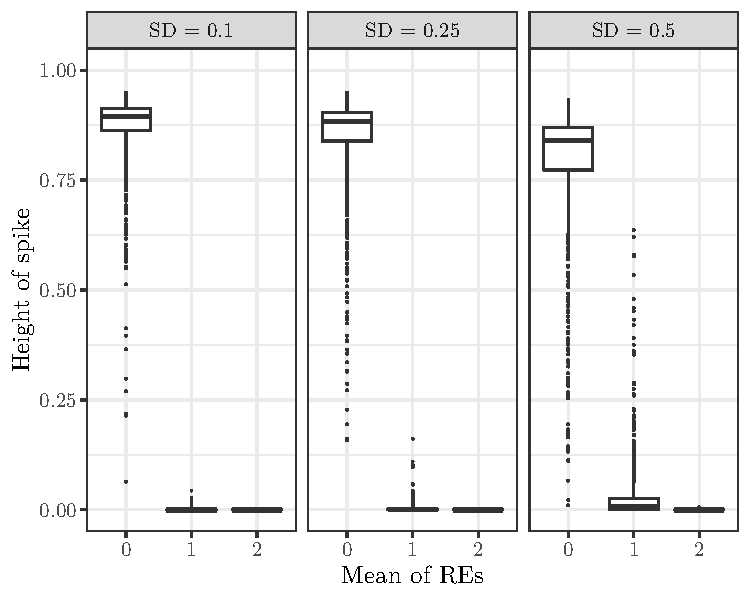
\includegraphics[height = 4in, width = 5in]{spike_boxplot.pdf}
\caption{Boxplots from Simulations 1 and 2: spike height for each combination of $\sigma_\delta$ and $\delta_0$}
\label{fig:SSP-boxplot}
\end{figure}

\begin{figure}
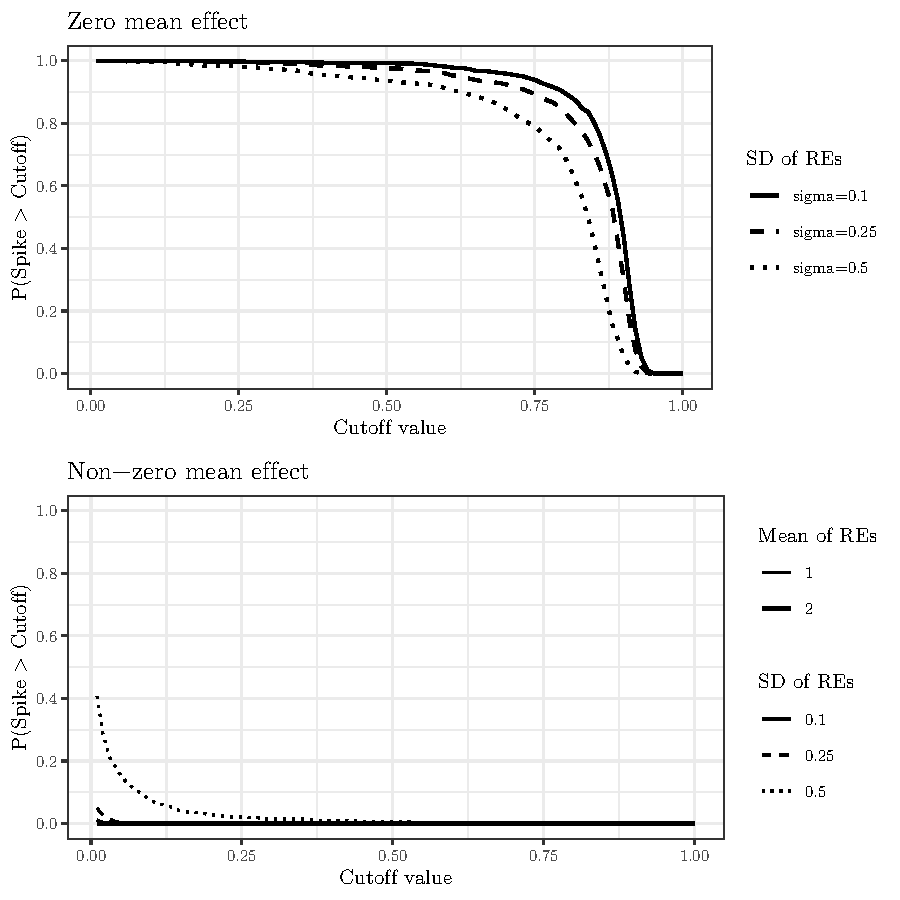
\includegraphics[height = 6in, width = 6in]{SSP-plot.pdf}
\caption{Top panel: proportion of Simulation 1 iterations where posterior spike height was higher than cutoff value with true zero mean effect.
Bottom panel: proportion of Simuation 2 iterations where posterior spike height was higher than cutoff value with true non-zero mean effect}
\label{fig:SSP-cutplot}
\end{figure}




\end{document}  